The core visual distinction is simple. A loop-centered agent treats messages,
tool logs, memory updates, usage, workspace effects, and branch provenance as
side channels around the loop. OpenRath moves those effects into one typed
runtime value. The same \texttt{Session} can be passed to agents, forked for
independent work, merged after review, persisted as evidence, and replayed with
explicit backend boundaries. OpenRath does not replace tool protocols, sandbox
providers, memory stores, tracing systems, or graph schedulers. It records
their effects in a session object that can move through the program as
branchable, inspectable, and replayable runtime state.

\begin{figure}[!htbp]
\centering
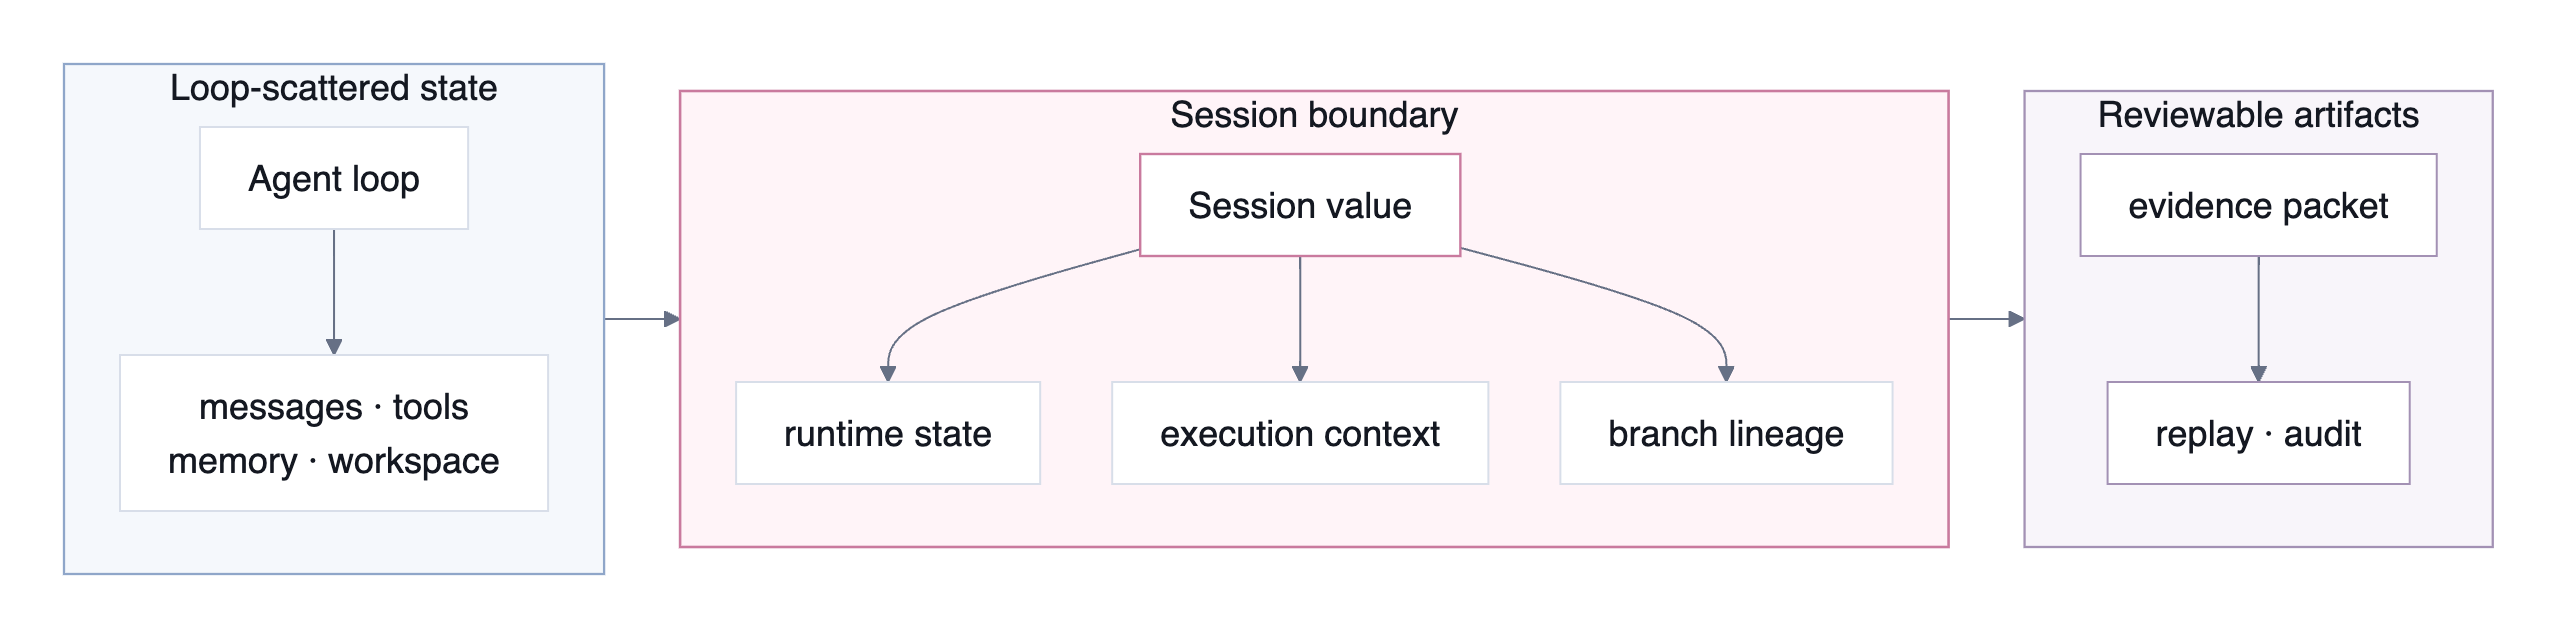
\includegraphics[width=0.96\linewidth]{assets/mermaid-diagrams/session-runtime-boundary.png}
\caption{OpenRath's core boundary: side-channel state around an agent loop is
promoted into a branchable \texttt{Session} value that can produce release
evidence artifacts.}
\label{fig:session-runtime-boundary}
\end{figure}
